\documentclass{IEEEtran}
\IEEEoverridecommandlockouts                             
\hyphenation{op-tical net-works semi-conduc-tor}

\usepackage{algorithm}
\usepackage{algpseudocode}
%\usepackage{acronym}
\usepackage{blindtext}
\usepackage[nolist]{acronym}
\usepackage[table, dvipsnames]{xcolor}
\usepackage[pdftex]{graphicx} % graphics package
\usepackage{graphicx}
\usepackage[colorinlistoftodos]{todonotes}
\usepackage{graphicx}
\usepackage{hyperref}

\usepackage{caption}
\usepackage{xcolor}
\usepackage{soul}
\captionsetup{compatibility=false}
\usepackage{subcaption}
\usepackage{array} % for defining custom column types
\usepackage{amssymb} %we added the package to the document
\usepackage[bottom]{footmisc}
\usepackage{booktabs}
\usepackage{amsthm}
\graphicspath{{figures/}} % declare the path where graphic files are
\DeclareGraphicsExtensions{.pdf,.jpg,.png} % grafic files extensions
\usepackage{amsmath} % math package for split
\usepackage{amsfonts} % math package for fonts
\usepackage{mathtools} % math package for tools like prescript
\usepackage{tikz} % figure package
\usetikzlibrary{shapes,arrows,fit,calc,positioning,automata,backgrounds}
%\usepackage{dblfloatfix} % figure package for positioning figures on the bottom
\usepackage{color} % colors package
\usepackage{multirow} % multiple rows in table
\usepackage{hhline} % separator in 
\usepackage{booktabs}
\usepackage[bookmarks=false, breaklinks]{hyperref} % hyperlink package
\usepackage{enumerate} % enumerate package
\usepackage{epstopdf} % package to include eps. files
\usepackage{dsfont}
\usepackage{textcomp}
\usepackage{algorithm}
\usepackage{algpseudocode}
\usepackage{siunitx} % package for international system units
\usepackage{cite}   % for compact citations, i.e. [1, 2]
\usepackage{diagbox}    % for making slash cell in a table
\usepackage{pdfpages}   
\usepackage{breqn}
\usepackage{svg}
\usepackage{multicol}
\svgpath{{images/svg/}} % <- using \svgpath to avoid warning
\colorlet{Green1}{green!90!}
\colorlet{Green2}{green!60!}
\colorlet{Green3}{green!40!}
\colorlet{Green4}{green!20!}
\colorlet{Green5}{green!10!}

% Used in order to break URL into smaller sections when seeing / or -
\usepackage{url}
\def\UrlBreaks{\do\/\do-}
\usepackage{breakurl}

%% ORCID
\RequirePackage{tikz} % For \foreach used for Orcid icon
% Make Orcid icon
\newcommand{\orcidicon}{\includegraphics[width=0.32cm]{images/orcid/logo-orcid.eps}}

% Define link and button for each author
\foreach \x in {A, ..., Z}{%
\expandafter\xdef\csname orcid\x\endcsname{\noexpand\href{https://orcid.org/\csname orcidauthor\x\endcsname}{\noexpand\orcidicon}}
}

\newcommand{\orcidauthorA}{0000-0001-5387-7613} % Add \orcidA{} behind the author's Hakim
\newcommand{\orcidauthorB}{0000-0003-3581-9481} % Add \orcidB{} behind the author's Olaya
\newcommand{\orcidauthorC}{0000-0002-1609-5783} % Add \orcidC{} behind the author's name  Halil
\newcommand{\orcidauthorD}{0000-0002-7742-6996} % Add \orcidD{} behind the author's name  Jonas
\newcommand{\orcidauthorE}{0009-0002-0445-8126} % Add \orcidE{} behind the author's name  Yury
\newcommand{\orcidauthorF}{0000-0002-7143-8777} % Add \orcidF{} behind the author's name  Erdal





\definecolor{Bookcolor}{HTML}{00F9DE}
\definecolor{darkgreen}{rgb}{0.0, 0.5, 0.0}
\definecolor{gray}{gray}{0.9}
\definecolor{lightgray}{rgb}{0.86, 0.86, 0.86}

\makeatletter
\def\@citex[#1]#2{\leavevmode
\let\@citea\@empty
\@cite{\@for\@citeb:=#2\do
{\@citea\def\@citea{,\penalty\@m\ }%
\edef\@citeb{\expandafter\@firstofone\@citeb\@empty}%
\if@filesw\immediate\write\@auxout{\string\citation{\@citeb}}\fi
\@ifundefined{b@\@citeb}{\hbox{\reset@font\bfseries ?}%
\G@refundefinedtrue
\@latex@warning
{Citation `\@citeb' on page \thepage \space undefined}}%
{\@cite@ofmt{\csname b@\@citeb\endcsname}}}}{#1}}
\makeatother


\newcommand{\HP}[1]{\textcolor{blue}{[HP: #1]}}
\newcommand{\HIU}[1]{\textcolor{red}{[HIU: #1]}}
\newcommand{\KA}[1]{\textcolor{orange}{[KA: #1]}}
\newcommand{\EK}[1]{\textcolor{magenta}{[EK: #1]}}
\newcommand{\JFS}[1]{\textcolor{darkgreen}{[JFS: #1]}}
\newcommand{\note}[1]{\textcolor{red}{[NOTE: #1]}}

\DeclareMathOperator*{\minimize}{{min}}
\DeclareMathOperator*{\maximize}{{max}}

\newcommand{\bm}[1]{\mathbf{#1}}

\newcommand{\orcidauthorA}{0000-0002-7742-6996} % Add \orcidA{} behind the author's name
\newcommand{\orcidauthorB}{0000-0002-7143-8777} % Add \orcidB{} behind the author's name
\begin{acronym}
    % \acro{CAMAP}{conflict-aware multi-agent planner}

    \acro{MPC}{model predictive control}
    \acro{GP}{Gaussian process}
    \acroplural{GP}[GPs]{Gaussian processes}
    \acro{AUV}{Autonomous underwater vehicle}
    \acro{MHE}{moving horizon estimator}
    \acro{ASGP}{adaptive sparse Gaussian process}
    \acro{EKF}{extended kalman filter}
    \acro{ROV}{remotely operated vehicle}
    \acro{DF-GP}{dynamic forgetting Gaussian process}
    \acro{IMU}{inertial measurement unit}
    \acro{DVL}{doppler velocity log}
    \acro{NED}{North-EastDown}
    \acro{RTI}{real-time iteration}
    \acro{NN}{neural network}
    \acro{OCP}{optimal control problem}
    \acro{LP}{linear program}
%    \acro{AUVs}{Autonomous underwater vehicles}
    \acro{ASGP}{adaptive sparse gaussian process}
    
\end{acronym}



\def\BibTeX{{\rm B\kern-.05em{\sc i\kern-.025em b}\kern-.08em
    T\kern-.1667em\lower.7ex\hbox{E}\kern-.125emX}}


\usepackage{amsthm}

\newtheorem{remark}{Remark}

    
\begin{document}
\title{ Empowering Autonomous Underwater Vehicles Using Learning-based Model Predictive Control With Dynamic Forgetting Gaussian Processes}


\author{Abdelhakim Amer, \IEEEmembership{Graduate Student Member, IEEE}, Mohit Mehndiratta, Yury Brodskiy and Erdal Kayacan, \IEEEmembership{Senior Member, IEEE}
% <-this % stops a space
\thanks{Submitted on July 5, 2024. This research receives support from Innovation Fund Denmark grant number 2040-00032B and EIVA a/s.}

\thanks{A. Amer is with the Artificial Intelligence in Robotics Laboratory (AiR Lab), Department of Electrical and Computer Engineering, Aarhus University, 8000 Aarhus C, Denmark {\tt\small abdelhakim@ece.au.dk}.}

\thanks{Mohit Mehndiratta is with GIM Robotics, Espoo, Finland, {\tt\small mohit.mehndiratta@gimrobotics.fi}.}


 \thanks{    Y. Brodskiy is with EIVA a/s, 8660 Skanderborg, Denmark. {\tt\small ybr@eiva.com.}}   
 
 \thanks{E. Kayacan is with the Automatic Control Group (RAT), Department of Electrical Engineering and Information Technology, Paderborn University, Paderborn, Germany. {\tt\small erdal.kayacan@uni-paderborn.de}.}%
}

\maketitle
\begin{abstract}

Autonomous underwater vehicles (AUVs) present several challenges due to the complex and simultaneous interplay of various factors, including but not limited to unmodeled dynamics, highly nonlinear behaviour, inter-couplings, communication delays, and environmental disturbances. In particular, environmental disturbances degrade trajectory tracking performance for model-based controllers, e.g., model predictive control (MPC) algorithms. Data-driven methods such as Gaussian process (GP) are effective at learning disturbances in real-time, however, the underlying offline hyperparameter tuning process limits their overall effectiveness. To overcome this limitation, we propose a novel dynamic forgetting Gaussian process (DF-GP) methodology that compensates for operational disturbances, thus circumventing the need for hyperparameter retuning. In essence, the proposed method optimally combines the predictions of individual GPs -- designed with handcrafted forgetting factors --, rendering precise disturbance estimation of varying timescales. What is more, the predicted disturbances update the model parameters in MPC, facilitating a learning-based control framework that ensures accurate tracking performance in different underwater scenarios. Rigorous simulation and real-world experiments demonstrate the efficiency and efficacy of the proposed framework. The results show a 25\% improvement in disturbance estimation and tracking performance, demonstrating that the proposed framework outperforms its direct competitors.%
\end{abstract}
\IEEEpeerreviewmaketitle

\begin{IEEEkeywords}
Autonomous underwater vehicle (AUV), model
predictive control (MPC), learning-based control, model learning, Gaussian processes (GPs), trajectory tracking.
\end{IEEEkeywords}


\section{Introduction}
\label{sec:introduction}

% % Underwater Robot Applications:
%
In many applications, \Acfp{ROV} play a pivotal role, including surveying, inspection, and search-and-rescue operations, by improving efficiency and ensuring safety \cite{amer2023unav, amergp}.
%
% Why We Need Tether:
%
Most \acp{ROV} are tethered to ensure a continuous power supply during long-duration missions and to maintain reliable communication.
%
% Introducing Problem Definition:
%
However, the presence of a tether introduces complexities in path planning and control, as it poses a risk of entanglement with underwater objects such as flora, fauna, or structures being inspected.

This challenge restricts the applicability of many path planning algorithms originally designed for untethered drones and surface vehicles. For instance, numerous \ac{CPP} algorithms exist to compute distance-optimal paths for covering 3D structures \cite{bircher2015structural,feng2024fc, amer2023visual}. Additionally, exploration path planners are employed to determine the next viewpoints for mapping and exploring unknown terrains \cite{dang2020graph}. However, these methods do not account for entanglement with the surroundings and thus cannot be directly applied to tethered underwater robots.
%
% Entanglement Problem and Definition:
%
Entanglement occurs when the movement of the underwater vehicle is restricted due to physical interactions between the tether and objects in the environment. Tether can bend or loop around obstacles, limiting vehicle mobility. This work bridges a critical gap in automatic asset inspection with \ac{ROV} by proposing \ac{REACT}.

The contributions of this work can be summarized as follows:
\begin{itemize}
\item A fast online tether model that computes the tether configuration in real time using \ac{SDF} data of arbitrary underwater structures.
\item An efficient online replanning method that prevents entanglement by incorporating a maximum tether length constraint.
\item Integration of the proposed method into a coverage path planning framework with \ac{MPC} to enable optimal inspection of underwater structures while avoiding entanglement.

\item Demonstration of the complete framework in simulation, showcasing its ability to ensure safe and efficient underwater structure inspection.
\end{itemize}





%
\begin{figure}[t!]
	\centering	\includegraphics[width=0.7\linewidth]{figures/react_abstract.pdf}
	  \caption{\textcolor{black}{Overview of the \ac{REACT} inspection framework. In the offline phase, a \ac{SDF} map is generated from a point cloud, and the FC-Planner \cite{feng2024fc} computes an optimal waypoint sequence. In the online phase, a tether model $\mathbf{P}^{tether}(t)$ ensures the maximum tether length is maintained, while an \ac{MPC} controller applies the optimal wrench $\mathbf{u}(t)$ to the \ac{ROV}}.}
    \label{fig:abstract}
\end{figure}
%


The remainder of this paper is organized as follows: Section \ref{sec:related_work} reviews the state of the art. Section \ref{sec:framework} presents the path planning framework for underwater structure inspection with tether constraints. Section \ref{sec:tether_model} introduces the taut-tether model, and Section \ref{sec:planner} details the online entanglement-aware path planner. Experimental results are shown in Section \ref{sec:experiments}, followed by conclusions and future work in Section \ref{sec:conclusion}.





 % 1 page

\section{State of the art}
\label{sec:related_work}

% Paragraph 1: Introduction to Tether Importance and Entanglement Definition
Tethers play a vital role in numerous mobile robotics applications, offering crucial power delivery and reliable data transmission. It enables extended operational periods and ensures consistent communication links for the robot. However, the risk of entanglement with obstacles represents a significant planning challenge. To systematically address this, a taxonomy of entanglement definitions has been presented in \cite{definitions}, cataloging existing interpretations from the literature and introducing new definitions, paving the way for developing new path planning strategies that account for entanglement.

% Paragraph 2: Early Approaches - 2D Offline Path Planning (Single Robot)
Initial efforts to develop entaglement-aware path planners often focused on two-dimensional environments and employed offline computation strategies. For instance, \cite{rov_mccammon} and \cite{mechsy2017novel} proposed methods for planning paths in 2D to cover a predefined set of waypoints while considering tether constraints. Notably, \cite{mechsy2017novel} formulated the path planning problem for a \ac{ROV} as a mixed-integer programming problem. Their approach first solves a \ac{TSP} to find an optimal waypoint sequence and then incorporates homotopic constraints during path generation to minimize the likelihood of tether entanglement. While effective for predefined scenarios, these offline methods lack the adaptability required for dynamic environments.

% Paragraph 3: Advancements - 2D Online Path Planning (Single Robot)
Addressing the need for real-time adaptability, subsequent research explored online path planning algorithms, still primarily in 2D. \cite{kim} introduced a homotopy-augmented topological approach combined with graph search techniques, allowing for dynamic adjustments to the path based on environmental perception. Similarly, \cite{withy} developed a hybrid A* variant that utilizes a modified tangent graph. This method efficiently plans curvature-constrained paths for tethered robots subject to winding angle constraints, demonstrating guarantees and providing simulation results for online entanglement avoidance. %These online planners represent a significant step towards real-time tether management.

% Paragraph 4: Scaling Complexity - Multi-Robot Systems in 2D
The complexity of tether management increases significantly when coordinating multiple robots. Several approaches have tackled this challenge in 2D. Early work by \cite{hert1996ties} laid groundwork in this area, followed by methods like \cite{zhang2019planning}. More recently, \cite{cao2023neptune} presented an efficient online path planner for multi-robot systems. Their method integrates a homotopy-based high-level planner with trajectory optimization and smoothing techniques to generate entanglement-free paths. However, despite its online capability, this approach remains constrained to 2D environments.

% Paragraph 5: Moving to Three Dimensions - 3D Path Planning (Single Robot)
Real-world applications frequently require navigation in 3D environments, such as with underwater robots. Consequently, work by  \cite{bhattacharya2012topological} and \cite{martinez2021optimization} explored topological aspects and optimization techniques for 3D tethered navigation. \cite{petit2022tape} specifically presented a 3D exploration path planner that incorporates explicit contact avoidance constraints for the tether, facilitating safer navigation for single tethered robots in complex three-dimensional spaces.

% Paragraph 6: 3D Multi-Robot Path Planning
 \cite{hert1999motion} extended their earlier 2D work to handle the increased complexity of 3D multi-robot scenarios. Further advancements by \cite{patil2023coordinating} and  \cite{cao2023path} introduced path planning strategies that explicitly consider the topological constraints imposed by multiple interacting tethers in 3D. While these methods advance the state-of-the-art in multi-robot coordination, they are generally designed for offline computation and are not suited for online path planning where real-time implementation is essential.

% Paragraph 7: Identifying the Research Gap
% Summarize the limitations of existing work: 
In summary, existing tether-aware planners often face limitations for practical online coverage path planning (CPP) in complex 3D settings. Many are too computationally intensive for real-time use \cite{mechsy2017novel, hert1999motion, patil2023coordinating, cao2023path}, lack integrated tether-aware CPP frameworks, or rely on simplifying assumptions like 2D environments or basic obstacle shapes \cite{kim, withy, cao2023neptune}, hindering generalization to real-world inspection tasks.
% Paragraph 8: Introducing the Proposed Solution (REACT) based on its key contributions
To address these limitations, we propose \ac{REACT}, a novel approach that enables real-time, entanglement-aware path planning in arbitrary 3-D environments.


% --- End of Literature Review Section ---













































% % Introduce tether in literature
% Tether considerations in autonomous robot planning has drawn increasingly attention in robotics literature due to their critical role in enabling robots to operate autonomously in unknown environments for a wide range of mobile robots. 
% % Entaglement definitions
% A taxonomy of entanglement definitions is presented in \cite{definitions} which catalogs existing definitions from the literature and also introduces six new definitions.  These definitions open the door to the design of new entanglement aware path planning approaches.

% % 2-D , offline
% Regarding the path planners, many path planning methods have been proposed to address tether entanglement in 2-D environments. \cite{rov_mccammon} and \cite{mechsy2017novel} propose 2-D offline path planning to cover a set a way-points. In particular, \cite{mechsy2017novel} formulate the path planning problem for a \ac{ROV} as a mixed-integer programming problem. Their method solves a \ac{TSP} to determine the optimal sequence of waypoint visits, while incorporating homotopic constraints to reduce the likelihood of tether entanglement.
% % 2-D , online
% Also in 2-D, but in an online fashion, a homotopy-augmented topological approach, combined with graph search techniques is proposed by \cite{kim}. In addition to offline methods, online path planners allow real-time entanglement avoidance \cite{kim}, \cite{withy}. A hybrid A* variant uses a modified tangent graph to efficiently plan curvature-constrained, tethered robot paths under winding angle constraints, with guarantees and simulation results provided \cite{withy}.
% % 2-D , Multirobot
% Other approaches, also in 2-D address the tether constraints problem for the multi-robot case in \cite{zhang2019planning}, \cite{hert1996ties}, and \cite{cao2023neptune}. An efficient online path planner is presented in \cite{cao2023neptune}, combining a homotopy-based high-level planner with trajectory optimization and smoothing to generate entanglement-free paths for multi-robot systems. However, this approach is limited to 2-D environments. 
% % 3-D , Multirobot
% Entanglement avoidance has also been investigated in 3-D environments, as demonstrated in \cite{petit2022tape}, \cite{martinez2021optimization}, and \cite{bhattacharya2012topological}. In particular, \cite{petit2022tape} presents a 3-D exploration path planner that incorporates contact avoidance constraints on the tether, enabling safe navigation for tethered robots in three-dimensional spaces. For multi-robot operations, \cite{hert1999motion} extends earlier work to handle the increased complexity of coordinating multiple tethered robots. Further advancements by \cite{patil2023coordinating} and \cite{cao2023path} introduce improved coordination strategies that consider topological constraints imposed by multiple tethers. However, these approaches are not designed for real-time, online path planning.

% % NICHE and summary of research gap 
% In summary, most existing planners suffer from limitations that hinder their use in practical, online coverage path planning applications. Many are too computationally intensive for real-time implementation, and there is a lack of coverage path planning frameworks that explicitly account for the tether during planning. Existing tether-aware methods often rely on simplifying assumptions, such as 2-D environments or simplistic obstacle shapes (e.g., circles or cylinders), and thus fail to generalize to complex, real-world environments—particularly in inspection tasks.
% % Introduce REACT
% To address these limitations, we propose \ac{REACT}, a novel approach that enables real-time, entanglement-aware path planning in arbitrary 3-D environments.

 % 1 page

\section{AUV Modelling}
\label{sec:model}


The equations of motion for the rigid body are described in a body-fixed coordinate system in the \ac{NED} frame (See Fig. \ref{fig:rov}) \cite{fossen}. Neglecting roll and pitch motion due to the restoring moment action significantly simplifies the equations of motion. This assumption, as adopted in \cite{shen2018path, heshmati2019robust}, enables more focus on the dominant dynamics of the system, which can be written as follows:

\begin{figure}[b!]
	\centering	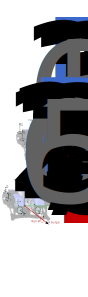
\includegraphics[width=0.7\linewidth]{figures/Introduction/brov.pdf}
	\caption{\ac{AUV} free body diagram and reference frames \cite{unav}.}
	\label{fig:rov}
\end{figure}


\begin{align}
\dot{x} &= \cos(\psi) u - \sin(\psi)  v \label{eq:xdot}\\
\dot{y} &= \sin(\psi)  u + \cos(\psi)  v \label{eq:ydot}\\
\dot{z} &= w \label{eq:zdot}
\end{align}
\begin{align}
(m - X_{\dot{u}})\dot{u} &= X + (m  v + Y_{\dot{v}}  v)  r \nonumber \\
&\quad + (X_u + X_{uc}  |u| )  u + \Delta_{x} \label{eq:udot}\\
(m - Y_{\dot{v}})\dot{v} &= Y - (m  u + X_{\dot{u}}  u)  r \nonumber \\
&\quad + (Y_v + Y_{vc}  |v|)  v + \Delta_{y} \label{eq:vdot}\\
(m - Z_{\dot{w}}) \dot{w} &= Z + (Z_w + Z_{wc}  |w|)w \nonumber \\
&\quad + m  g - V_{sub} \rho_{water}  + \Delta_{z}\label{eq:wdot}\\
\dot{\psi} &= r \label{eq:psidot}\\
(I_{zz} - N_{\dot{r}}) \dot{r} &= M_z - (m  v - Y_{\dot{v}}  v)  u \nonumber \\
&\quad - (X_{\dot{u}}  u - m  u)  v  \nonumber \\
&\quad + (N_r + N_{rc}  |r|)  r + \Delta_{M_z} \label{eq:rdot}
\end{align}

In the equations above, the translational positions $x$, $y$, and $z$ are specified within the earth-fixed frame $\mathcal{F}_E$. The translational velocities $u$, $v$, and $w$ are represented in the body frame $\mathcal{F}_B$, whereas $r$ denotes the rotational velocity about the z-direction. Translational velocities in $\mathcal{F}_E$ can be obtained by rotating the body velocities with an angle $\psi$ about the heave direction. The vehicle's mass is denoted by $m$, the angular moment of inertia about the z-axis is denoted as $I_{zz}$, $g$ describes the gravitational constant, $\rho_{water}$ is the water density, and $V_{sub}$ denotes the total submerged volume. $X$, $Y$, and $Z$ denote applied wrenches by actuators acting on the \ac{AUV} body in $\mathcal{F}_B$, while $M_z$ represents the externally applied moment about the z-axis. Here, $\mathbf{\Delta}  \in \mathbb{R}^{4}$ given by [$\Delta_{x}$, $\Delta_{y}$, $\Delta_{z}$ $\Delta_{M_z}$] are the external disturbances affecting the \ac{AUV} body in the body frame. This term accounts for the lumped unmodeled disturbances arising from currents, tether, and other effects.


The parameters $X_{\dot{u}}$, $Y_{\dot{v}}$, $Z_{\dot{w}}$, and $N_{\dot{r}}$ represent added mass parameters. $X_{u}$, $Y_{v}$, $Z_{w}$, and $N_{r}$, as well as $X_{uc}$, $Y_{vc}$, $Z_{wc}$, and $N_{rc}$, denotes linear and quadratic drag coefficients about the surge, sway, heave, and yaw directions, respectively. The parameters for the BlueROV2 heavy model, used for both simulation and controller model, are provided in Table \ref{tab:brovparams}. The equations of motion can also be rewritten in state-space form:



\begin{table*}[t]
\caption{BlueROV2 heavy parameters}
\centering
\normalsize
\setlength{\tabcolsep}{4pt} % Adjust column spacing if needed
\renewcommand{\arraystretch}{1.5} % Adjust row height (1.0 is normal}
\begin{tabular}{|c|c|c|c|c|c|c|c|c|c|c|c|c|c|c|}
\hline
$X_{\dot{u}}$ & $Y_{\dot{v}}$ & $Z_{\dot{w}}$ & $N_{\dot{r}}$ & 
$X_{u}$ & $Y_{v}$ & $Z_{w}$ & $N_{r}$ & $X_{uc}$ & $Y_{vc}$ & $Z_{wc}$ & $N_{rc}$ & $m$ & $V_{sub}$ & $I_{zz}$ \\ \hline
-2.6 & -18.5 & -13.3 & -0.28 & 
-0.09 & -0.26 & -0.19 & -4.64 & -34.9 & -103.25 & -74.2 & -0.43 & 11.4 & 115 & 0.24 \\ \hline
\end{tabular}

\label{tab:brovparams}
\vspace{-0.3cm}
\end{table*}

%
\begin{align} \label{eq:model_eqs}
    \dot{\mathbf{x}} = \mathtt{f}(\mathbf{x}_k,\mathbf{u}_k, \mathbf{\Delta}),  \quad
   % \mathtt{z}_k = \mathtt{h}(\mathtt{x}_k,\mathtt{u}_k),
\end{align}
%
 The vectors $\mathbf{x} \in \mathbb{R}^{8}$ and $\mathbf{u} \in \mathbb{R}^{4}$  denote the state and control vectors, respectively
%
\begin{align}
\label{eq:state_control} 
    \mathbf{x} &= [x,y,z,u,v,w, \psi, r]^T, \quad  \\
    \label{eq:control} 
    \mathbf{u} &= [X,Y,Z,M_z]^T.
\end{align}
%
The state transition function is represented by $\mathtt{f}(\cdot,\cdot, \cdot)$: $\mathbb{R}^{8} \times \mathbb{R}^{4} \times 
 \mathbb{R}^{4} \rightarrow \mathbb{R}^{8}$.

 
%\begin{align} \label{eq:state_trans}
%   \textcolor{red}{ \mathtt{f}(\mathbf{x}_k,\mathbf{u}_k) = %\mathbf{x}_k + \Delta t \hspace{0.1cm}  \dot{\mathbf{x}_k}}
   % \mathtt{z}_k = \mathtt{h}(\mathtt{x}_k,\mathtt{u}_k),
%\end{align}.

%\textcolor{red}{where $\Delta t$ is the time step.}

















 



 

 % 1.5 pages
\section{Model Predictive Control}
\label{sec:mpc}


%{MPC}'s exceptional success lies in its distinctive capacity to manage constraints, along with a myriad of other design specifications, while optimizing performance systematically and elegantly through iterative online optimization processes \cite{ Mohit2017Receding, mpc_survey, vtnmpc}. This method is also called receding horizon control. The optimal control problem is given in discrete time as follows:




\ac{MPC} is an optimization-based control strategy aimed at determining an optimal sequence of actions over a predefined time horizon, denoted by $N_c$. This optimization process is conducted at each time step in a receding horizon manner after the system's initial state is updated. The optimal control problem is given in discrete time as follows:
%
{
\begin{subequations} 
\label{eq:NMPC}
\begin{align}
    \minimize_{\mathbf{x}_k,\mathbf{u}_k} \quad & \sum_{k = 0}^{N_c-1} \left( \|\mathbf{x}_k- \mathbf{x}^{ref}_k\|^2_{\mathbf{Q}}
    +  \|\mathbf{u}_k\|^2_{\mathbf{R}}\right) + 
    \nonumber
    %\\
    %&\quad \hspace{4cm}    
    \|\mathbf{x}_ {N_c}- \mathbf{x}^{ref}_{N_c}\|^2_{\mathbf{Q}_T} \nonumber \\
    & \label{eq:NMPC1} \\
    \text{s.t.} \quad & \mathbf{x}_{k+1} = \mathtt{f}_d(\mathbf{x}_k,\mathbf{u}_k, \mathbf{\Delta}) , \quad k \in [0, N_c-1],  \nonumber \\
    & \label{eq:NMPC2} \\
    & \mathbf{u}_{k,\textrm{l}} \leq \mathbf{u}_k \leq \mathbf{u}_{k,\textrm{u}}, \quad k \in [0, N_c-1].  & \label{eq:NMPC4} 
\end{align}
\end{subequations}
}
%
The discretized nonlinear model, denoted as $\mathtt{f}_d(\mathbf{x}_k, \mathbf{u}_k, \mathbf{\Delta})$, is obtained by applying a 4th-order Runge-Kutta method to the continuous dynamics in \eqref{eq:model_eqs}. The equations are discretized using a chosen sampling time $T_s$. Additionally, a zero-order hold assumption is adopted for the control inputs, whereby the control inputs $\mathbf{u}$ remain constant throughout each sampling interval $T_s$.

Herein, $\mathbf{u}_{k,\textrm{l}}$ and $\mathbf{u}_{k,\textrm{u}}$ denote the respective minimum and maximum bounds on the controls, where each is a vector in $\mathbb{R}^{4}$. The components inside the summation in \eqref{eq:NMPC1} represent costs associated with the full state and control vectors \eqref{eq:state_control} and \eqref{eq:control}. While the state cost penalizes the deviations between the predicted $\mathbf{x}_k$  and reference $\mathbf{x}^{ref}$ states, the control cost minimizes energy consumption along the trajectory. The second term in \eqref{eq:NMPC1} is the terminal cost, which caters to the finite nature of the prediction horizon, thereby ensuring convergence.  In this context, $ \mathbf{Q} \in \mathbb{R}^ {8 \times 8} $, $  \mathbf{Q}_{T} \in \mathbb{R}^ {8 \times 8}$,  and $  \mathbf{R} \in \mathbb{R}^ {4 \times 4} $ are positive-(semi) definite weight matrices. In this work, we obtain the coefficients of the weight matrices using the meta-heuristic strategy described in \cite{mpc_tune}.


 % 0.5 pages
\section{Dynamic Forgetting Gaussian Process}
\label{sec:dfgp}
In this section, we elaborate on the overall \ac{DF-GP} methodology proposed in this work. We begin with summarizing the nominal dense \ac{GP} expressions, followed by the \ac{ASGP} method proposed in \cite{asgp}. Then, we illustrate the implementation details of the online \ac{ASGP} method along with the adopted GP architecture. Finally, we deduce the optimization problem of the \ac{DF-GP} methodology and establish its global convergence.


\subsection{Gaussian process preliminaries}
In essence, a \ac{GP} is a set of infinitely-dimensional random variables characterized by a joint Gaussian probability distribution \cite{williams2006gaussian}. 
Let there be  data set $\mathbf{D}$ of size $n$ given by
%
\begin{equation} \label{eq:data}
  D_i = \bigl\{\mathbf{a}_i, y_i\bigl\}, \hspace{0.5cm}   i \in [1, n],
\end{equation}
%
where $\mathbf{a}_i$  $\in \mathbb{R}^d$ and $y_i$ are the input-target of observations, with $d$ representing the input dimensionality. The goal is to estimate an unknown function $f(\mathbf{a}_i)$ that maps the inputs $\mathbf{a}_i$ to the target $\mathbf{y}_i$:
%
\begin{equation} \label{eq:data}
  y_i =f(\mathbf{a}_i)+\epsilon_i, \hspace{0.5cm}    \epsilon_i \sim \mathcal{N}(0,\,\sigma_{\varepsilon_{i}}^{2}),
\end{equation}
where $\epsilon_i$ is an additive white noise, with a variance $\sigma_{\varepsilon_{i}}^{2}$. For simplicity, we will henceforth omit the index $i$. A prior on the underlying function can be deduced, such that $f(\mathbf{a})$ forms a \ac{GP} defined by a mean function $m(\mathbf{a})$ and covariance kernel $k(\mathbf{a},\mathbf{a}')$.


 %Gaussian processes (GP) is probabilistic regression method for approximating nonlinear function, $f\left(\bullet\right):\mathbb{R}^{D}\to\mathbb{R}$. It takes in some input-output pairs $\mathbb{D}$
%\begin{notation}$\bm{x}\in\mathbb{R}^{D}$  $y\in\mathbb{R}$ is the measurement of $f\left(\bm{x}\right)$, i.e., $y=f\left(\bm{x}\right)+\varepsilon$, where $\varepsilon\sim\mathcal{N}\left(0,\sigma^2_\varepsilon\right)$ is the Gaussian noise; $\sigma^2_\varepsilon\in\mathbb{R}^+$ is the noise variance.	Assuming that a dataset $\left\{\bm{x}_n,y_n\right\}_{n=1}^N$ is collected. Let $f_n$ denotes $f\left(\bm{x}_n\right)$ abbreviatedly; define compact forms $\bm{X}_N=\left\{\bm{x}_n\right\}_{n=1}^N\in\mathbb{R}^{N\times D}$, $\bm{y}_N=\left\{y_n\right\}_{n=1}^N\in\mathbb{R}^{N}$, $\bm{f}_N=\left\{f_n\right\}_{n=1}^N\in\mathbb{R}^{N}$.\end{notation}

%\\
%A prediction $f_*=f\left(\bm{a}_*\right)$ at a test point $\bm{a}_*$, assuming that vector $\bm{y}$, which represnts the vetcor of target [y1, . . . , yN ] and $f_*$ have a joint Gaussian distribution given as:
A prediction \(f_* = f\left(\bm{a}_*\right)\) at a test point \(\bm{a}_*\) assumes that the vector of target values \(\bm{y} = [y_1, \dots, y_n]^\top\) and the prediction \(f_*\) have a joint Gaussian distribution given by:



\begin{equation}
	\begin{bmatrix}
		\bm{y} \\ f_*
	\end{bmatrix}
	\sim
	\mathcal{N}
	\left(\bm{0},
	\begin{footnotesize}\begin{bmatrix}
			\bm{K}_{aa}+\sigma^2_\varepsilon\bm{I} & \bm{k}_{a*} \\
			\bm{k}_{*a} & k_{**}
	\end{bmatrix}\end{footnotesize}\right),\label{eq:p_jointx}
\end{equation}
with the covariance calculated using a squared exponential kernel, as follows:
\begin{equation}
	\hspace{-1.9mm} k\left(\bm{a},\bm{a}'\right)= \sigma_f^2\exp\left(-\frac{1}{2}\left(\bm{a}-\bm{a}'\right)^T\bm{L}_a^{-2}\left(\bm{a}-\bm{a}'\right)\right),\label{kernal}
\end{equation}
wherein $\sigma_f^2$ $\in$ $\mathbb{R}^+$  denote the prior variance, and $\bm{L}_a\in\mathbb{R}_{>0}$ is a diagonal matrix that represents the input length scales. Together, these parameters form the kernel hyperparameters \(\theta \in \mathbb{R}^{d+1}\), which determine the  characteristics of the functions that the \ac{GP} samples from. Typically, the optimal hyperparameters, \(\theta_{\text{opt}}\), are obtained by minimizing the negative log marginal likelihood represented as follows: 
%
\begin{equation} \label{eq:hyper_opt}
    \theta_{\text{opt}} = \arg \min_{\theta} \left( \frac{1}{2} \mathbf{y}^T \bm{K}_{aa}^{-1} \mathbf{y} + \frac{1}{2} \log |\bm{K}_{aa}| + \frac{n}{2} \log 2\pi \right).
\end{equation}
%
Finally, the joint probability distribution \eqref{eq:p_jointx} is conditioned  on $\bm{y}$ to calculate the posterior distribution of $f_{*}$, resulting in the following posterior prediction equations for the test point $\bm{a}_*$:
\begin{align}
%	&p\left(f_*|\bm{y}\right) = \mathcal{N}\left(\mu_*, \Sigma_*\right) \label{eq:pred_dense1}\\
	&\mu_* = \bm{k}_{*a}\left(\bm{K}_{aa}+\sigma^2_\varepsilon\bm{I}\right)^{-1}\bm{y}, \label{eq:pred_dense2}\\
	&\Sigma_* = k_{**} - \bm{k}_{*a}\left(\bm{K}_{aa}+\sigma^2_\varepsilon\bm{I}\right)^{-1}\bm{k}_{a*}. \label{eq:pred_dense3}
\end{align}

 
\subsection{Adaptive sparse Gaussian process}
%Next, we introduce the \ac{ASGP} as proposed in \cite{asgp}: 
A recent work in \cite{asgp} introduces an adaptive version of the variational sparse GP method, referred to as the \ac{ASGP}, which utilizes the following mean and variance equations:
%
\begin{align}
	\mu_*(\lambda) &= \sigma^{-2}_\varepsilon\bm{k}_{*s}\bm{B}_\lambda\bm{K}_{sa}\bm{\Lambda}\bm{y}, \label{eq:pred_asgp1}\\
	\Sigma_*(\lambda) &= k_{**} + \bm{k}_{*s}\left(\bm{B}_\lambda-\bm{K}_{ss}^{-1}\right)\bm{k}_{s*}, \label{eq:pred_asgp2}
\end{align}
%
where $\bm{\Lambda}$ (forgetting factor matrix) and $\bm{B}_\lambda$ are expressed as:
%
\begin{align}
	\bm{\Lambda} &= {\rm diag}\left(
	\begin{matrix}
		\lambda^{n-1} & \lambda^{n-2} & \cdots & \lambda^0
	\end{matrix}\right), \label{eq:pred_asgp3}\\
	\bm{B}_\lambda &= \left(\bm{K}_{ss}+\sigma^{-2}_\varepsilon\bm{K}_{sa}\bm{\Lambda}\bm{K}_{as}\right)^{-1}. \label{eq:pred_asgp4}
\end{align}
%
The equations above utilize a vector of inducing points \( \mathbf{s}_m \), where \( m \in \{1, \ldots, M\} \). There are \( M \) such inducing points, which together provide a sparse approximation of the dense input \( \mathbf{a} \), enabling computationally efficient and real-time prediction capabilities. Furthermore, introducing a forgetting factor enables prediction equations tailored for time-series data. This factor prioritizes recent data points with exponentially increasing weights, emphasizing recent data in the prediction. %Furthermore, since it comprises a sparse covariance matrix $\bm{K}_{ss}$, it enables computationally efficient and real-time prediction capabilities.


%Furthermore, the equations rely on sparsification approximation, of the \ac{GP}, enabling more efficient implementation and real-time prediction capabilities.


 
 
\subsection{Online ASGP for disturbance prediction}

Next, we describe the procedure for generating the data set $ D = \bigl\{\mathbf{a}, y\bigl\}$, which is used by the \ac{ASGP} for predicting the disturbance at the following time step ($\hat{\Delta}_{t+1} = \mu_*(\lambda)$). At an arbitrary measurement time $\tau$, the input vector and target scalar are defined in the following manner:  
%
\begin{align} \label{eq:gp_data}
 %\mathbf{a} &= [ \Delta_{t-h}, \mathbf{x}_{t-h}, \mathbf{u}_{t-h}]  , \; \forall h = 0, \cdots, H \\
\mathbf{a} &= [ \Delta_{\tau-1-H}, \mathbf{x}_{\tau-1-H}, \mathbf{u}_{\tau-1-H}, \cdots, \Delta_{\tau-1}, \mathbf{x}_{\tau-1}, \mathbf{u}_{\tau-1}], \\
y &=  \Delta_{\tau}. \label{eq:input_target}
\end{align}
%
The input vector $\mathbf{a}$ is constructed utilizing the historical data, wherein $H$ represents the length of the data history. 
%contains a history of disturbance estimates $\Delta_{t-h}$, where $H$ represents the length of the data history. 
The disturbance value at time instance $\tau$ ($\Delta_{\tau}$) is computed from the model equations \eqref{eq:model_eqs}, by incorporating the corresponding acceleration and velocity feedback along with the control input. %Then, \ac{GP} uses this historical data to predict the disturbance at the next time instance, i.e., $\hat{\Delta}_{t+1}$.

It is important to note that there is a one-time step difference between the input and output to facilitate learning. This input-output choice renders the \ac{GP} model more effective in learning disturbances. Also, the feature space is augmented with states and control inputs to embed the associated dynamics information. Moreover, a separate \ac{GP} model is employed for disturbance estimation along each axis to streamline the input space and reduce computational complexity. Furthermore, the dataset is partitioned into two sets as proposed in \cite{mohit_gp}, namely $D^1$ and $D^2$. The static dataset $D^1$, collected at the beginning of the operation, is utilized for hyperparameter optimization. On the other hand, the dynamic dataset $D^2$ is updated online, wherein the latest acquired data point replaces the first element (oldest data point). This design allows the forgetting factor to balance between the offline collected dataset $D^1$, representing nominal model errors, and the online collected dataset $D^2$, representing sudden disturbances, such as currents.


%\begin{remark}
%\textcolor{red}{The partitioning of the dataset is based on the following rationale: Dataset D1 represents a nominal dataset that captures historical modeling errors under standard operating conditions, primarily encompassing recurring unmodeled effects. In contrast, Dataset D2 consists of more recent, online-collected data that includes sudden and abrupt disturbances encountered during operation.By using both datasets, we can balance the forgetting factor ($\lambda$) to appropriately weigh the influence of older nominal disturbances (from D1) against the impact of newer, sudden disturbances (from D2). This approach helps in managing the computational burden of the MPC algorithm by ensuring that the model remains responsive to recent changes while still incorporating valuable historical data. For more detailed information on this approach, please refer to \cite{mohit_gp}}
%\end{remark}


%The input vector $\mathbf{a} $ contains a history of disturbance estimates $\Delta_{t-j}$, where $J$ represents the length of the data history. It is important to note that there exists a one-time step difference between the input and output to facilitate learning. This input-output choice aids the \ac{GP} in more effectively learning disturbances. Moreover, the feature space is augmented by incorporating state and control input. To streamline the input space and reduce computational complexity, a separate \ac{GP} for disturbance estimation along each axis.
%Furthermore, the dataset is partitioned into two sets as described in \cite{mohit}: $D^1$ and $D^2$. $D^1$ is a static dataset collected at the beginning of the operation, which is also used for hyperparameter optimization. The dataset $D^2$ is dynamic, updated online where the first element (oldest) is replaced with the newest acquired data. This design allows the forgetting factor to balance between the offline collected dataset $D^1$, representing nominal model errors, and the online data collected $D^2$, representing sudden disturbances such as currents.




\subsection{Dynamic weight optimization}


As mentioned earlier, the forgetting factor in the \ac{ASGP} formulation can be crucial in time-series data prediction, making it suitable for predicting rapidly changing disturbances. However, a critical challenge lies in determining the optimal value for this factor. One potential approach is to choose the forgetting factor that maximizes the log-likelihood. However, this method can be computationally demanding and may struggle to adapt effectively to dynamic datasets.


 To address the limitation above, a dynamic forgetting approach is proposed to effectively weigh the predictions from multiple \ac{GP} models with varying forgetting factors. The formulation of the proposed optimization problem is as follows:
%
\begin{subequations} \label{eq:DF}
\begin{align}
	\minimize_{{\eta}_j} \quad & \sum_{j = 1}^{K} \sum_{i = 1}^{N} {\eta}_j  \|\mu^{j}_{*t-i-1}(\lambda_j)- \Delta_{t-i}\|^{2}_{\alpha_i}, \
 %{\alpha}_i \left( \mu^{k}_{i} - y_{i}\right)
 % \|\mu^{k}_{i}- y_{i}\|^{2}  
  \label{eq:DF1} \\
    	\textrm{s.t.} \quad & \sum_{j = 1}^{K} {\eta}_j = 1 , \hspace{0.2cm} j \in [1, K],  &   \label{eq:DF2} \\
    &  {\eta}_j \geq 0 , \hspace{0.8cm} j \in [1, K]. &   \label{eq:DF2} 
\end{align}
\end{subequations}
%
Here, \(K\) denotes the number of \ac{GP} models used in the prediction, where $K$ is a user-defined number. In essence, the objective is to obtain the optimal weights ($\eta_{j}$) that minimize the Euclidian error between the individual GP prediction ($\mu_{*t-i-1}^{j}(\lambda_j)$) and the corresponding measured disturbance values ($\Delta_{t-i}$). %It is to be noted that subscript $*$ in \eqref{eq:DF1} indicates the inference at the test point $\bm{a}_*$ and is included to establish notational consistency with \eqref{eq:pred_asgp1}.  
%
%
%\begin{remark}
%\textcolor{red}{ TODO: differentate lambda and alpha. keywords: lambda weights the data points contrubution within mean computation. whereas, alphai wheights the contriubtion of different costs () for optimizing lambda value (make better, comment 4 reviewer 3).The exponential relationship for $\alpha_i$ is chosen to give higher importance to more recent errors compared to older ones. This ensures that the model places greater emphasis on correcting recent prediction errors, which is crucial for maintaining accurate and adaptive predictions. If $\alpha_i$ were the same for each $i$, it would imply equal weighting of all past errors, regardless of their recency. This would diminish the ability of the model to adapt to recent changes or trends in the data, potentially reducing its effectiveness in capturing the latest dynamics of the system.}
%\end{remark}
%
Note that the optimization problem in \eqref{eq:DF1} is solved over a historical measurement horizon comprising $N$ data points. This measurement horizon ensures that the weighted combination results in higher prediction accuracy over consecutive time points, rather than just the current time, rendering a stable optimal solution. As such, $N$ can be inferred as a critical parameter that substantially influences the optimization process. Opting for a small $N$ might hinder the ability of the \ac{GP} model to capture past effects, i.e., making it near-sighted, thereby rendering overemphasis on the recent data. Conversely, selecting a large $N$ introduces computational burdens and reduces the responsiveness of the \ac{GP} model to recent disturbances.
%


%\begin{remark}
%    \textcolor{red}{Although the ASGP will try to minimize the error associated with the cost function \eqref{eq:DF} through predictions at the next time step \(\mu_{*t}\), there will inevitably be some discrepancy due to the inherent limitations of the GP’s prediction capabilities. Therefore, it is necessary to optimize the weights \(\eta\) to determine which ASGPs, with the respective forgetting factor $\lambda$, are most effective at minimizing this prediction error, considering disturbances. }
%\end{remark}



Additionally, $\alpha_i$ represents the relative weightage of \ac{GP} prediction errors within the $N$-point horizon. Intuitively, an exponential expression $\alpha_i = e^{0.05 (N - i)}$ is defined. Exponential weighting via $\alpha_i$ allows the model to prioritize recent data, improving its ability to track fast-changing disturbances. For instance, if $\alpha_i$ is set as unity, the model will treat all past errors equally, reducing its adaptability to recent disturbances. To maintain consistency among \ac{GP} model predictions, the constraints in \eqref{eq:DF1} and \eqref{eq:DF2} are introduced.



%This approach ensures that the predictions derived from multiple \ac{GP} models are effectively aligned with the historical data while considering the impact of past observations on the prediction accuracy.

\begin{remark}
It is important to distinguish between $\alpha_i$ and the the forgetting factor $\lambda$: while $\lambda$ determines the contribution of historical data points in the \ac{GP} mean computation, \(\alpha_i\) weighs the different prediction-error terms over the measurement horizon \(N\) in the optimization process for the weights \(\eta\). 
\end{remark}



%\begin{remark}
%\textcolor{red}{
%The optimization of the forgetting factor is a low-dimensional problem, with the dimensionality ($K$) typically being less than 10. }
%\end{remark}

The overall learning-based MPC framework, as depicted in Fig. \ref{fig:abstract}. Furthermore, A pseudo-code for the overall frame is provided in algorithm~\ref{alg:dynamic_forgetting_gp}. Note that the algorithm is presented for a single dimension of the \ac{GP}. The same procedure is applied independently to the x, y, and z directions to learn disturbances along each respective axis.



%% Algorithm starts here
%%%
\begin{algorithm}
\caption{Dynamic Forgetting Gaussian Process (DF-GP)}\label{alg:dynamic_forgetting_gp}
\begin{algorithmic}[1]
\State \textbf{Input:} 
\Statex \quad Measurement horizon \(H\)
\Statex \quad Number of \ac{GP} models \(K\)
\Statex \quad Forgetting factors \(\lambda_j\)
\vspace{0.2cm}
\State  Generate datasets \(D^1\) and \(D^2\), incorporating \eqref{eq:gp_data},\eqref{eq:input_target}
\State  Optimize GP hyperparameters, using \eqref{eq:hyper_opt}
\vspace{0.2cm}

\While{learning is active}

    \State \quad Get current state and control
    \State \quad Update \(D^2\), append new data and remove old
    \For{ each GP model with \(\lambda_j\)}
        \State \quadCompute predictions \(\mu_{gpj}\), using \eqref{eq:pred_asgp1}
    \EndFor
    \State \quad Optimize weights \(\eta^{opt}\) over horizon \(N\), using \eqref{eq:DF}
    \State \quad {Predict disturbance \(\hat{\Delta}_{t+1}\) with \(\eta^{opt}\) using \eqref{eq:pred_dfgp1}.
    \State \quad {Update MPC model with \(\hat{\Delta}_{t+1}\), using \eqref{eq:NMPC1}
\EndWhile
\end{algorithmic}
\end{algorithm}






\subsubsection*{Feasibility and optimality} 

To analyze the feasibility and  (global) optimality, the optimization problem in \eqref{eq:DF} can be represented in the following standard form:
%
\begin{subequations} \label{eq:LP}
\begin{align}
	\minimize_{\boldsymbol{{\eta}}}\quad & \boldsymbol{c}^{T}{\boldsymbol{\eta}} \label{eq:LP1}  , \\
   	\textrm{s.t.} \quad & \boldsymbol{a}^{T}  {\boldsymbol{\eta}}  = b \  &   \label{eq:LP2} \\
    &  \boldsymbol{{\eta}} \geq \boldsymbol{0}, \label{eq:LP3} 
\end{align}
\end{subequations}
%
where \eqref{eq:LP1} defines the cost function with the coefficient vector $\bm{c} \in\mathbb{R}^{K\times 1}$ written as follows:  
 \begin{align*}
    \mathbf{c} = 
      \begin{bmatrix} 
        \sum_{i = 1}^{N} \alpha_i(\mu^1_{t-i-1} - \Delta_{t-i})^2 \\
        \sum_{i = 1}^{N} \alpha_i(\mu^2_{t-i-1} - \Delta_{t-i})^2 \\
        \vdots \\
        \sum_{i = 1}^{N} \alpha_i(\mu^K_{t-i-1} - \Delta_{t-i})^2 \\
      \end{bmatrix} \in\mathbb{R}^{K\times 1}  \neq \mathbf{0},
 \end{align*}
and \eqref{eq:LP2} and \eqref{eq:LP3} represent the underlying constraints with the following variable definitions:
\begin{align*}
    \boldsymbol{a} = \begin{bmatrix} 
      \mathbb{I} 
    \end{bmatrix} \in\mathbb{R}^{K\times 1} , \quad
    b = 1,
\end{align*}
wherein $\mathbb{I}$ infers an identity vector. This formulation is clearly a \ac{LP} due to its affine objective and constraint functions, demonstrating the convex nature of the problem.
%
%With a closer look at \eqref{eq:LP}, one may identify its similarity to a linear program due to the underlying affine objective and constraint functions. This infers the convex nature of the posed optimization problem while assuming the boundedness of $\mu_{*\tau}^{j}$ and $\Delta_{\tau}$ at the time instant $\tau$.
Given the inherent convexity of linear programs, global convergence to the optimal solution is ensured, assuming feasibility. Efficient \ac{LP} solvers can thus reliably solve this problem.


%Consequently, the global convergence of its solution can be ensured by selecting efficient \ac{LP} solvers. 


\begin{remark}
The optimization problem in \eqref{eq:LP} is a linear program that guarantees the existence of a solution. Non-uniqueness may occur if the vector $\mathbf{c}$ contains identical or zero elements. However, in most practical scenarios where $K$ is a small integer, a unique solution is typically achieved while ensuring feasibility.
\end{remark}





%\begin{remark}
%\textcolor{red}{Since the optimization problem in \eqref{eq:LP} is a linear problem that typically provides a solution, especially given the low dimensionality (e.g., \(K=3\) in Section VI). The only scenario where the LP might fail is if \(\mathbf{c} = 0\) or all elements of \(\mathbf{c}\) are equal, leading to a non-unique solution. However, this is highly unlikely, ensuring the feasibility of the problem in almost all cases.}
%\end{remark}




\begin{figure}[t]
	\centering	\includegraphics[width=1.0\linewidth]{figures/Introduction/new_abstract.pdf}
	\caption{ The proposed learning-based \ac{MPC} framework. }

%	\caption{First,  \ac{GP} models with varying forgetting factors $\lambda_i$ are utilized to generate  predictions of the disturbances $\mu_{gpj}$. Dynamic weight optimization is then performed, where the optimal weight $\eta^{opt}$ of each prediction is obtained, to minimize the error between $N$ measurements $\Delta_{t-i}$ and the \ac{GP} predictions. These optimal weights are then used to predict the disturbance at the next time instance $\hat{\Delta}_{t+1}$, updating the \ac{MPC} model.  }
 
	\label{fig:abstract}
\end{figure}


%$\boldsymbol{A}$ is the constraint matrix, which is an identity vector of size $1 \times K$, and $\boldsymbol{b}$ is the constraint vector , which is an identity matrix size $1 \times 1$. 

%It should be noted that the current optimization problem is posed as \ac{LP} in standard form \cite{boyd2004convex}, which implies convexity and hence global convergence using standard efficient \ac{LP} solvers. 




The obtained optimal weights $\eta^{opt}_j$ are then utilized to obtain a new prediction equation for the \ac{DF-GP} as follows: 
\begin{align} 
	\mu_{*DF} &= \displaystyle\sum_{j=1}^{K} \eta^{opt}_j \mu_{*t}(\lambda_j) , \label{eq:pred_dfgp1}\\
	\Sigma_{*DF} &=  \displaystyle\sum_{j=1}^{K} \eta^{opt}_j \Sigma_{*t}(\lambda_j). \label{eq:pred_dfgp2}
\end{align}









%We define the Linear program in standard form as in \cite{boyd2004convex},  $\eta \in \mathbb{R}^{K},$ where $A$ $\in \mathbb{R}^{1\times K}$ and $b$ is $\mathbb{I}$ and  $\in  \mathbb{R}^{1\times 1}$. $c^{T}_{i}$ is $\in \mathbb{R}^{1\times K},$ and is equal $[\alpha_i(\mu^j_i-\Delta_{i})^2 ]$ where j \in [0, K],. % 0.25 page
\section{Experimental results}
\label{sec:expirments}
The algorithm's predictive accuracy and trajectory tracking capabilities are assessed against state-of-the-art benchmarks through simulations and indoor pool testing.

\subsection{Implementation details}



The scenario is simulated using the underwater robotic simulator, Mobula \footnote{https://www.eiva.com/products/navisuite/navisuite-bundles/navisuite-mobula-pro-videoray}. 
The inducing points are chosen to be identical to the inputs for consistency between the different methods. The first ten seconds of data are recorded for training the \ac{GP}, where the conjugate gradient method is employed to optimize the hyperparameters. Regarding implementing the proposed \ac{DF-GP} approach, we set $K$ to be three, which implies solving the optimization problem \eqref{eq:DF} for three \ac{GP}s with forgetting factors namely, $1$, $0.8$, and $0.6$.  
%for consistently with the baselines. 
As such, the number of selected \ac{GP} models is a user-defined configuration parameter. While adding more \ac{GP} models is expected to enhance performance, it also increases the computational burden. Additionally, the measurement horizon $N$ is set to 20 samples which is determined via the trial-and-error method. Moreover, the \ac{DF-GP} method is implemented using the CasADi  \cite{casadi}. For the \ac{MPC}, which is used as the tracking controller with all the \ac{GP} models, a direct multiple shooting method with a $0.05$-second grid size is used. The solution is obtained via solving a sequential quadratic program with a combination of the generalized Gauss-Newton method and the real-time iteration scheme. ACADO toolkit \cite{acado} and qpOASES solver \cite{qpoases} handle the solution for \eqref{eq:NMPC}, with $N_c = 100$ prediction horizon and $0.05$ second sampling time. A long horizon was selected which ensures accurate tracking, improved safety, and reliable constraint satisfaction.








\subsection{Simulation experiments}

%describe simulation scenario
% - whats the trajectory, disturbances, implementation details, other methods to compare.
% disturbance estimation of different algorithms, error etc.
% weights plots
% trajectory tracking vs MPC



%comment on the performance 
%\begin{equation}
%    \text{disturbance} = 
%    \begin{cases}
%     \text{sine}(t)\, &   t < 30 \\
%      \text{sine}(t) + \text{cos}(t) + \text{sine}(2t), & t<55
%    \end{cases}
%    \label{eq:dist}
%\end{equation}


  




A lemniscate trajectory, comprising two cycles, is provided as a reference to the \ac{MPC}, while the scenario includes the introduction of a disturbance profile consisting of a sine wave, a combined sine wave (combination of different sine waves as included in \cite{mohit_gp}), and a square wave. 
We first motivate the inclusion of a dynamic forgetting factor by implementing our method with fixed forgetting values, namely $\lambda = 1.0$, $\lambda = 0.8$, and $\lambda = 0.6$. Additionally, four different baselines are implemented: an \ac{MPC} without a \ac{GP}, the \ac{GP}-\ac{MPC} method proposed in \cite{mohit_gp}, the fast adaptive sparse \ac{GP} (Fast-AGP) proposed in \cite{asgp}, the \ac{MHE} disturbance observer augmented with \ac{MPC} proposed in \cite{mpc_mhe}, and finally, the proposed method, \ac{DF-GP}. Moreover, we also test the \ac{MPC} without disturbances to illustrate the best-case tracking performance.



%Furthermore, four different baselines are implemented: a \ac{MPC} without a \ac{GP}, \ac{GP}-\ac{MPC} method proposed in \cite{mohit_gp}, the fast adaptive sparse \ac{GP} (Fast-AGP) proposed in \cite{asgp}, \textcolor{red}{the \ac{MHE} disturbance observer augmented with \ac{MPC} proposed in \cite{mpc_mhe}} and finally the proposed method, \ac{DF-GP}. Furthermore, we also test the \ac{MPC} without disturbances to illustrate the best-case tracking performance. 



%For the \ac{MPC} implementation, the direct multiple shooting method is utilized with a shooting grid size of $0.05$ seconds. Consequently, the resulting discretized \ac{OCP} reduces to a sequential quadratic program, which is solved via the generalized Gauss-Newton method with \ac{RTI} scheme \cite{DIEHL2002577}. ACADO toolkit \cite{acado}, along with the qpOASES solver \cite{qpoases}, is chosen as the solution platform for solving the OCP in \eqref{eq:NMPC}, as it incorporates the direct multiple shooting method and the RTI approach altogether. Additionally, the prediction horizon $N_c = 100$ and a sampling time of $0.05$ seconds are specified.








The overall performance enhancement of the \ac{DF-GP} compared to other methods is illustrated in Table \ref{tab:sim}. 
%
\begin{table}[b]
  \caption{Simulation results summary: The \ac{DF-GP} method demonstrates significant improvements in prediction compared to baselines. The improvement percentage is calculated relative to the GP-MPC method in disturbance prediction and relative to the \ac{MPC} with no \ac{GP} in tracking performance.}
  \centering
  \footnotesize % Decrease font size for the whole table
  \begin{tabular}{|>{\centering\arraybackslash}p{1.9cm}|>{\centering\arraybackslash}p{1.1cm}|>{\centering\arraybackslash}p{0.8cm}|>{\centering\arraybackslash}p{1.cm}|>{\centering\arraybackslash}p{0.8cm}|>{\centering\arraybackslash}p{0.6cm}|} % Compute column is now last
    \hline
    Method & Mean prediction error [$m/s^2$] & Improve. \%  & Mean traj. error [m] & Improve. \%  & \textcolor{black}{Comp. [ms]} \\ % Compute is now the last column
    \hline
    \textit{Ideal} &  -    &  -   &    \textit{0.0186}  &   \textit{82.3} & - \\
    No GP   &  -      &  -   &    0.105  &  0.0 & - \\
    \textcolor{black}{MHE-MPC \cite{mpc_mhe}} & \textcolor{black}{0.445}  & \textcolor{black}{37.8}  & \textcolor{black}{ 0.0889}  & \textcolor{black}{15.3}  & \textcolor{black}{2.41} \\
    GP-MPC \cite{mohit_gp}  & 0.716  &  0.0  &    0.0597   &  43.1 & \textcolor{black}{1.25}  \\
    Fast-AGP \cite{asgp} &  0.381 & 46.8  &  0.0378     & 64.0 & \textcolor{black}{0.748}  \\    
    $\lambda = 1.0$ & 0.644  &   10.1 & 0.0519 &  50.6 & 0.788  \\
    $\lambda = 0.8$ &0.674  &   5.97 & 0.0505 & 51.9 & \textbf{0.720} \\
    $\lambda = 0.6$ & 0.656    & 8.38   &0.0514& 51.0 &\textcolor{black}{0.756}  \\
    DF-GP           & \textbf{0.289} &  \textbf{59.6}   & \textbf{0.0285}  & \textbf{72.9} &  2.05 \\  
    \hline
  \end{tabular}  

  \label{tab:sim}
\end{table}
Particularly, regarding the motivation for dynamic forgetting compared to a static forgetting factor, while a fixed forgetting factor provides a prediction error of about $0.66$ $m/s^2$, the \ac{DF-GP} outperforms it by reducing the prediction error to less than half, i.e., to $0.289$ $m/s^2$. The reason is that a fixed forgetting factor is not suitable for different disturbance scenarios. Initially, when the disturbance is repeated, a higher $\lambda$ value renders a large dataset which is crucial for accurate prediction. Conversely, when the disturbance profile abruptly changes, such as in combined disturbances or square wave cases, a lower $\lambda$ is needed as older data becomes less relevant and recent data gains importance. The \ac{DF-GP} method strikes a balance as it weights different \ac{GP} models and quickly adapts predictions based on the error of each model within a short horizon.



 Figure \ref{fig:prediction} illustrates the disturbance profile alongside the predictions generated by GP model from different methods. 
 %
 \begin{figure}[t]
	\centering	\includegraphics[width=0.95\linewidth]{figures/Simulations/pred_mhe.pdf}
	\caption{\ac{GP} predictions during the simulation run. \ac{DF-GP} effectively predicts the disturbance profile by optimally combining contributions from different \ac{GP}s.}
	\label{fig:prediction}
\end{figure}
%
\begin{figure}[b]
	\centering	\includegraphics[width=1\linewidth]{figures/Simulations/pred_err_mhe.pdf}
	\caption{\ac{GP} predictions error in simulation for the \ac{GP} with different forgetting factors. The \ac{DF-GP} method maintains low prediction errors. }
	\label{fig:pred_error}
\end{figure}
 %
 \begin{figure}[t]
	\centering
	\includegraphics[width=1\linewidth]{figures/Simulations/lem_mhe.pdf}
	%\includegraphics[width=0.97\linewidth]{figures/Simulations/traj2.pdf}
	\caption{Obtained trajectory in simulation for the proposed \ac{DF-GP} method against baselines. }%By accurately learning disturbances of varying magnitude and frequencies, \ac{DF-GP} method outperforms the baselines in the trajectory tracking task achieving comparable performance to the ideal (no disturbance) scenario. Points indicating the initiation of different disturbance profiles are highlighted in blue.}
	\label{fig:traj}
\end{figure}
 %
 Up until the first 30 seconds, all  \ac{GP}s are able to predict the disturbance profile relatively well. Starting at time $t=30$, the disturbance profile shifts to a combined sine wave, where the GP-MPC \cite{mohit_gp} is failing to follow the profile, as it has not encountered it before in the training data. On the other hand, the Fast-AGP and \ac{DF-GP} are able to accurately follow the disturbance profile, even as it switches. This can be attributed to the forgetting factor and the dynamic selection of inducing points in \cite{asgp}. Notably, our \ac{DF-GP} method demonstrates a superior ability to quickly adapt to the changing disturbance profile and maintain accuracy, as evidenced by the error plot in Fig. \ref{fig:pred_error}. This capability is due to its innovative approach of balancing multiple predictions by optimizing the weights of these predictions, enabling it to dynamically adjust and respond to the changing disturbance profile.

%However, we can clearly observe the ability of the DF-GP method to quickly adapt to the disturbance profile and accurately follow it as shown in the error plot in Fig. \ref{fig:pred_error}. This can be attributed to its ability to balance different predictions by optimizing weights of different predictions.







\begin{figure}[t]
	\centering	\includegraphics[width=0.90\linewidth]{figures/Simulations/traj_err_mhe.pdf}
	\caption{Trajectory tracking error results. The peaks in the error correspond to when the disturbance profile changes and the applied disturbance reaches a maximum magnitude.} %The \ac{DF-GP} method consistently outperforms baselines throughout the trajectory, after applying three different disturbance profiles. }
	\label{fig:traj_error}
\end{figure}








Figure \ref{fig:traj} presents the tracking accuracy of the \ac{DF-GP} method compared to the baselines \ac{MPC}. It is evident that \ac{DF-GP} outperforms baselines in terms of tracking precision.  Figure \ref{fig:traj_error} showcases the trajectory tracking errors, with mean errors depicted for each forgetting factor. The enhancement in disturbance prediction translates into improved tracking accuracy for \ac{DF-GP}, demonstrating superior performance compared to other methodologies. Furthermore, the \ac{MHE}-\ac{MPC} demonstrated worse tracking performance than \ac{DF-GP} method, primarily due to the lack of predictive capability. Additionally, the computational performance of the methods is shown in \ref{tab:sim}. As expected, the methods based on \ac{ASGP} are the fastest, as they rely on quick online updates of new data points and dynamic inducing point selection. They are followed by the \ac{GP}-\ac{MPC} method, which uses a dense \ac{GP} implementation. The proposed \ac{DF-GP} method is not far behind; it only requires additional computation for \eqref{eq:DF}, which is an \ac{LP} with $K$ = 3, adding just 0.8 ms to the \ac{GP} predictions. Thanks to the efficient C++ implementation, which utilizes multithreading and parallelization, adding multiple \ac{GP} predictions did not noticeably increase the computation time. On the other hand, the \ac{MHE}-\ac{MPC} method had a higher computational cost, as it relies on a more expensive nonlinear optimization problem over a past horizon. 



\subsection{Real-world experiments }
\label{sec:real}
%To further validate the simulation results, a real-world experiment is conducted at EIVA experimental test facility, in a $3 \times 5 \times 4$ pool, where the simulation test scenario is replicated.
To enhance the validation of the simulation results, a real-world experiment is carried out at the EIVA experimental test facility, utilizing a 3 × 5 × 4 meter pool \footnote{The authors would like to thank Adis Hodzic, Ernest Wilk, Mathias Friis Spaniel, and Thomas Frank Klein from EIVA for their help with the experimental setup.}.  The motivation to conduct real-world tests is twofold:

\begin{enumerate}
    \item To demonstrate real-time feasibility, including computational feasibility and communication delays.
    \item To showcase the effectiveness of the framework against unmodeled real-time effects, wall effects, self-induced currents by the \textcolor{black}{\ac{AUV}}, and tether.
\end{enumerate}
The experiment is conducted with a circular reference trajectory of 1-meter diameter due to space limitations. A BlueROV2 Heavy equipped with a BlueRobotics Navigator board \footnote{https://bluerobotics.com/store/comm-control-power/control/navigator/}, which incorporates an \textcolor{black}{\ac{IMU}}, compass and barometer is utilized. These sensors measure acceleration, heading, depth, and attitude estimates. Furthermore, a Wayfinder Doppler velocity log\footnote{https://www.teledynemarine.com/en-us/products/Pages/Wayfinder.aspx} is used to obtain the velocity estimate. The pose estimates are then derived through dead-reckoning based on the obtained velocities. To introduce periodic disturbances, the \ac{AUV} tether is tied to one side of the pool, creating a challenging environment for the \ac{AUV}.  %The obtained \ac{AUV} trajectories are shown in Figs. \ref{fig:error-real} and \ref{fig:pred_dist_real}. 
%\begin{figure}[!htb]
%	\centering	\includegraphics[width=0.95\linewidth]{figures/Expirements/traj_real.pdf}
%	\caption{Obtained trajectory in real-world experiments for the proposed \ac{DF-GP} method against nominal \ac{MPC} method.}
%	\label{fig:traj-real}
%\end{figure}
Figures \ref{fig:error-real} and \ref{fig:pred_dist_real} demonstrate that the \ac{DF-GP} strategy can learn the unmodelled effects of the inaccuracies and achieve a better trajectory tracking accuracy than nominal \ac{MPC} by improving the tracking error by $34.5\%$. This allows for learning unmodeled disturbances, such as tether effects, \ac{AUV}-generated currents, thrust degradation, and other factors.


\begin{figure}[t]
	\centering	\includegraphics[width=1.0\linewidth]{figures/Expirements/error_real.pdf}
	\caption{Trajectory error obtained in real experiments for  \ac{DF-GP} and nominal \ac{MPC}. Dynamic disturbance learning through \ac{DF-GP} enhances tracking performance significantly.}
	\label{fig:error-real}
\end{figure}


\begin{figure}[t]
	\centering	\includegraphics[width=1.0\linewidth]{figures/Expirements/pred_real.pdf}
	\caption{Comparison of real-world test predictions against disturbance calculations (pseudo-ground truth).} %The pseudo-ground truth is obtained by calculating disturbances at the current time instance \(\Delta_t\) using the system model equations. The first 15 seconds are used for collecting the training data and hyperparameter optimization of the \ac{GP}.}
	\label{fig:pred_dist_real}
\end{figure}







 % 0.25 page
%\input{sections/7-real-time-expirements} % 0.25 page
%\section{Acknowledgement}
%The authors thank Adis Hodsic, Ernest Wilk, Mathias Spaniel, and Thomas Klein (EIVA) for experimental support.










\section{Conclusion}
\label{sec:conclusion}

%In this study, a learning-based \ac{MPC} framework was introduced, which leverages \ac{DF-GP} to address rapidly changing and difficult-to-model disturbances encountered in underwater robotics. 
This study introduces a learning-based \ac{MPC} framework that utilizes \ac{DF-GP} to effectively predict disturbances of varying magnitude and frequencies encountered in underwater robotics. This framework facilitates the integration of various \ac{GP} contributions, ensuring its applicability across different scenarios without the necessity for hyperparameter retuning during operation. Furthermore, the global convergence of the proposed method is analyzed. The conducted experiments demonstrate a \(59.6\%\) improvement in disturbance estimation accuracy and a \(72.9\%\) enhancement in tracking performance across various disturbance profiles. Overall, the results validate that the proposed framework outperforms its direct competitors, achieving a \(25\%\) improvement in both disturbance estimation and tracking performance. Future studies will explore the impact of dynamic input and inducing point selection. %for a fully automated learning-based \ac{MPC} framework.
 % 0.25 page

\bibliographystyle{IEEEtran}

\bibliography{References.bib}

\end{document}
